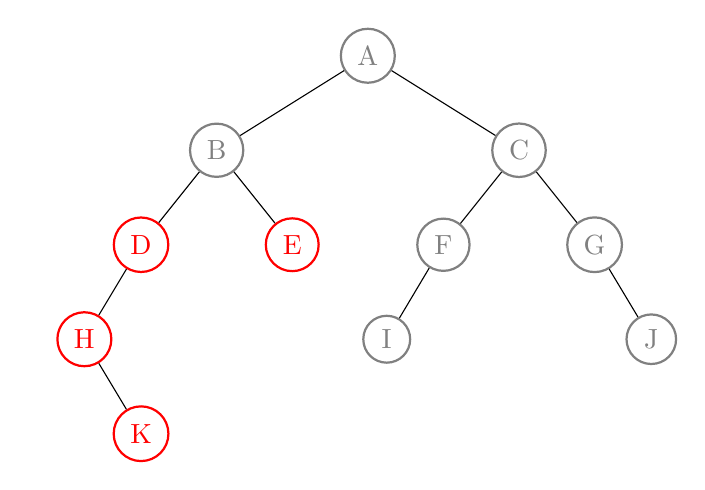
\begin{tikzpicture}[scale=0.8]

  %% \tikzstyle{every node}=[ball color=red!70,circle,text=white]

  %% \node [circle,draw] at (0,0) {A}; 

  \node[gray,thick,circle,draw] at (0,0) {A}[sibling distance=4.8cm] 
  child { node[gray,thick,circle,draw]{B}[sibling distance=2.4cm]
    child {node[red,thick,circle,draw]{D}[sibling distance=1.8cm]
      child {node[red,thick,circle,draw]{H}
        child[fill=none] {edge from parent[draw=none]}  
        child {node[red,thick,circle,draw]{K}}
      }
      child[fill=none] {edge from parent[draw=none]}  
    }
    child {node[red,thick,circle,draw]{E}}
  }
  child { node[gray,thick,circle,draw]{C}[sibling distance=2.4cm]
    child {node[gray,thick,circle,draw]{F}[sibling distance=1.8cm]
      child {node[gray,thick,circle,draw]{I}}
      child[fill=none] {edge from parent[draw=none]}  
    }
    child {node[gray,thick,circle,draw]{G}[sibling distance=1.8cm]
      child[fill=none] {edge from parent[draw=none]}  
      child {node[gray,thick,circle,draw]{J}}
    }          			
  };
 
  
\end{tikzpicture}
